\documentclass[times, utf8, seminar]{fer}
\usepackage{booktabs}
\usepackage{amstex}
\usepackage{hyperref}
\usepackage{listings}
\usepackage{color}

\setcitestyle{square}
\definecolor{dkgreen}{rgb}{0,0.6,0}
\definecolor{gray}{rgb}{0.5,0.5,0.5}
\definecolor{mauve}{rgb}{0.58,0,0.82}

\lstset{frame=tb,
    language=Java,
    aboveskip=3mm,
    belowskip=3mm,
    showstringspaces=false,
    columns=flexible,
    basicstyle={\small\ttfamily},
    numbers=none,
    numberstyle=\tiny\color{gray},
    keywordstyle=\color{blue},
    commentstyle=\color{dkgreen},
    stringstyle=\color{mauve},
    breaklines=true,
    breakatwhitespace=true,
    tabsize=3
}


\begin{document}
    \tableofcontents
    %! Author = Dean
%! Date = 12/16/2023

\chapter{Uvod}\label{ch:uvod}
U današnje vrijeme generira se iznimna količina podataka, pogotovo vizualnih podataka kao što su slike na društvenim mrežama pa sve do
medicinskih snimaka, a najveći izazov je otkriti korisne informacije.
Upravo u tom kontekstu, konvolucijske neuronske mreže (KNM) izronile su kao ključni model u svijetu računalnog vida.
Seminar započinje pregledom osnova neuronskih mreža.
Zatim, obrađene su razne teme vezane za KNM, poput arhitekture, glavnih komponenata, način treniranja i optimizacije te uporaba u stvarnom svijetu.
    %! Author = Dean
%! Date = 12/16/2023


\chapter{Neuronske mreže}\label{ch:neuronske-mreze}

Neuronske mreže čine podskup strojnog učenja i predstavljaju temelj algoritama dubokog učenja.
Inspiracija za strukturu i način rada neuronskih mreža crpi se iz ljudskog mozga pokušavajući oponašazi biološke neurone i njihovu međusobnu komunikaciju.


\section{Umjetni neuron}\label{sec:umjetni-neuron}
Prvi model umjetnog neurona je razvijen od strane Warrena McCullocha i Waltera Pittsa, poznat kao McCulloch-Pitts
model umjetnog neurona. Ovaj model oponaša funkcionalnost biološkog neurona, gdje ulazni signali utječu na odluku neurona o tome hoće li
se on aktivirati ili ne
McCulloch-Pitts model umjetnog neurona sastoji se od \textit{n} ulaznih značajki ili signala, označenih s $x_1, x_2, \dots, x_n$, te njihovim pripadajućim težinama $w_1, w_2, \dots, w_n$ koje određuju važnost pojedinih informacija.
\FloatBarrier
\begin{figure}[h]
    \centering
    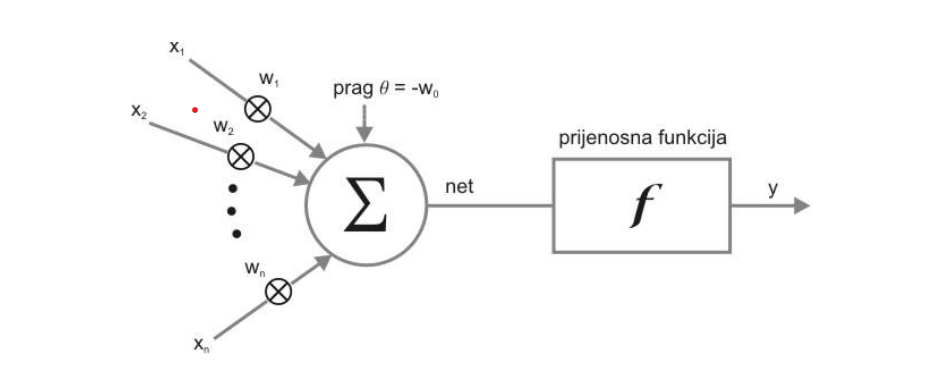
\includegraphics[width=0.8\textwidth]{images/Umjetni_neuron}
    \caption{McCulloch-Pitts model umjetnog neurona%
    \protect\footnotemark}
    \label{fig:slika1}
\end{figure}
\FloatBarrier
\footnotetext{\url{https://www.fer.unizg.hr/_download/repository/UmjetneNeuronskeMreze.pdf}}

Težinska suma neurona \emph{net} se izračunava kao suma ulaznih značajki
\[ net = x_0*w_0 + x_1*w_1 + \dots + x_n*w_n \]
Gdje nam $w_0$ označava takozvana vrijednost praga \emph(bias) koji služi kako bismo odredili kada će neuron biti aktivan ili ne.
Dok nam $x_0$ služi samo radi lakšeg matematičkog zapisa i on je uvijek jedank 1. Znajući sve ovo sad možemo težinsku sumu napisati kao
\[ net = \sum_{i=0}^{\n} w_0*x_0 \]
Drugi način težinske sume koristi vekotorski oblik
\[ net =\vec{w}^T \cdot \vec{x} \]
Na kraju \textit{net} propustimo kroz takozvanu aktivacijsku funckiju \textit{f} koja će nam dati izlaz.

\subsection{Aktivacijska funkcija}\label{subsec:aktivacijska-funkcija}
Aktivacijska funkcija je funkcija koja nam daje izlaz neurona na temelju težinske sume.
Glavna uloga aktivacijske funkcije je ta što ona odlučuje hoće li neuron biti aktivan ili ne ili bolje rečeno hoće neuron u toj situaciji biti
važan u ulozi predikcije.
Najjednostavnija moguća aktivacijska funkcija je funkcija identiteta
\[ f(\textit{net}) = net \]
Danas najčešće korištene aktivacijske funkcije us sigmoidalna u ReLU.
Sigmoidalna funkcija je definirana kao:
\[ f(\textit{net}) = \frac{1}{1 + e^-net} \]
\FloatBarrier
\begin{figure}[h]
    \centering
    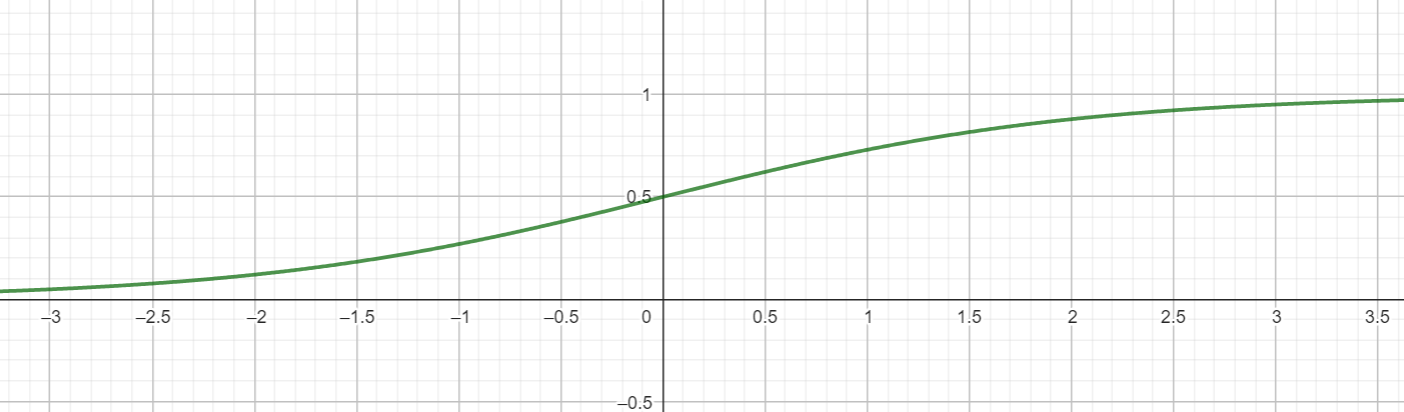
\includegraphics[width=0.8\textwidth]{images/Sigmoid}
    \caption{Sigmoidalna funkcija}
    \label{fig:slika2}
\end{figure}
\FloatBarrier
Kodomena sigmoidalne funkcije je (0, 1) gdje će za jako velike vrijednosti težiti ka 1 a za jako male vrijednosti težiti ka 0.
ReLU aktivacijska funkcija je definirana kao:
\[ f(\textit{net}) = \max(0, \textit{net}) \]
\FloatBarrier
\begin{figure}[h]
    \centering
    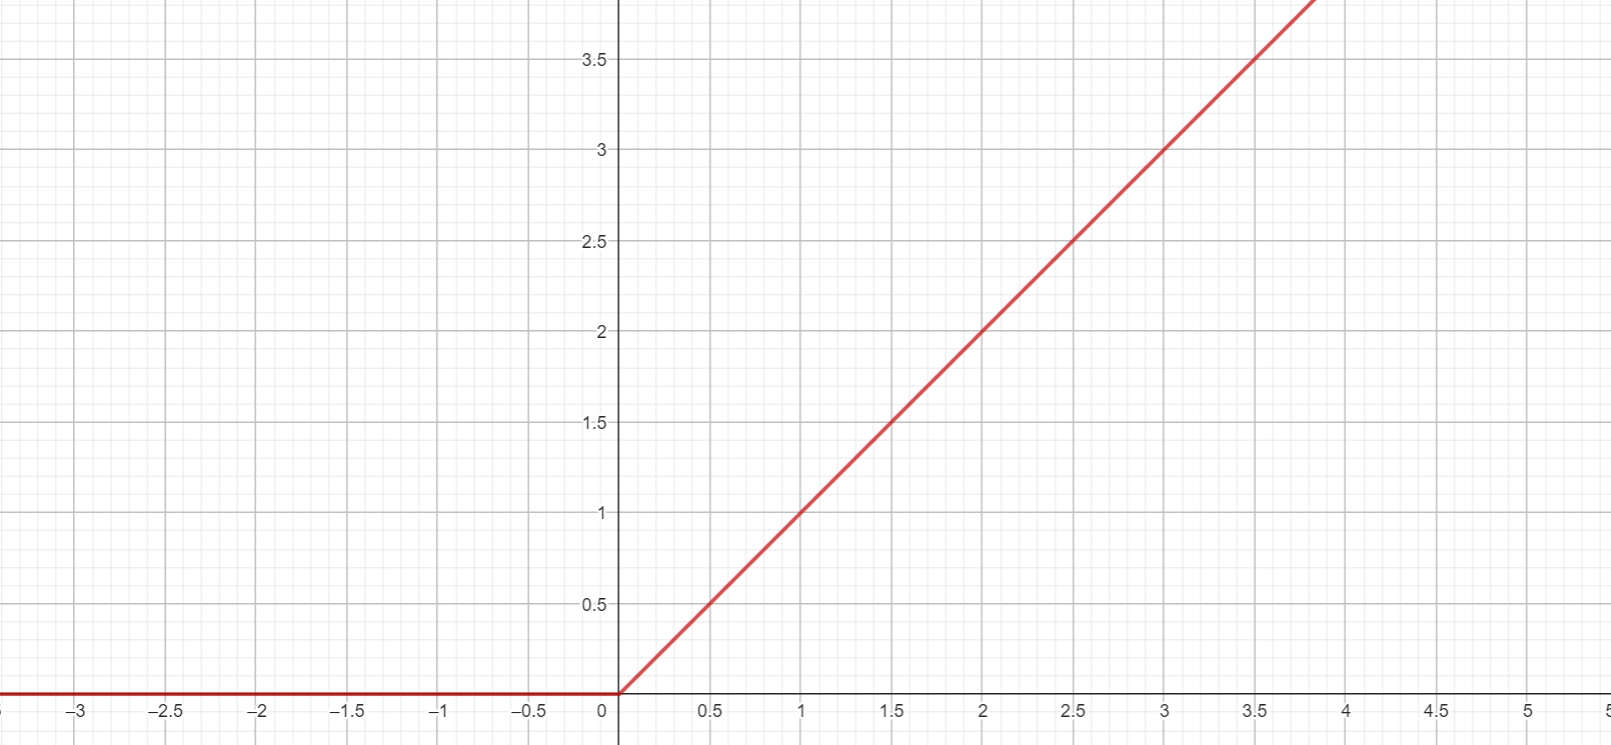
\includegraphics[width=0.8\textwidth]{images/ReLU}
    \caption{ReLU}
    \label{fig:slika3}
\end{figure}
\FloatBarrier


\section{Višeslojne neuronske mreže}\label{sec:viseslojne-neuronske-mreze}

\subsection{Struktura mreže}\label{subsec:struktura-mreze}
Način na koji su neuroni međusobno povezani i organizirani u mreži određuju njezinu arhitekturu te razlikujemo 4 osnovne arhitekture:

\begin{enumerate}
    \item aciklička mreža
    \item mreža s povratnom vezom
    \item lateralno povezana mreža
    \item hibridne mreže
\end{enumerate}

AcIklička mreža nema povratnih veza između neurona tako da je propagacija signala jednosmjerna.
Kod ovakvih vrsta mreža razlikujemo ulazni sloj neurona, skriveni sloj neurona i izlazni sloj neurona.
Ulazni sloj neurona nemaju ulazne signale odnosno nemaju ulogu neurona već samo propagiraju signal iz ulaznog sloja u prvi skriveni sloj.
Skriveni sloj se sastoji od jednog ili više sloja neurona.
Skriveni slojevi igraju ključnu ulogu u procesu učenja i ekstrakciji značajki iz podataka.
I na kraju imamo izlazni sloj koji sadrži rezultat.
\FloatBarrier
\begin{figure}[h]
    \centering
    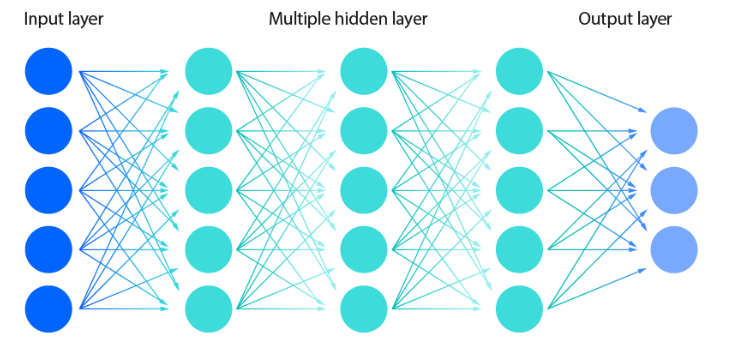
\includegraphics[width=0.8\textwidth]{images/nn-arch}
    \caption{Aciklička mreža
    \protect\footnotemark}
    \label{fig:slika4}
\end{figure}
\FloatBarrier

\footnotetext{\url{https://www.ibm.com/topics/neural-networks}}

Neuronske mreže s povratnom vezom sadrže u svojoj strukturi barem jednu povratnu vezu.
Što znači da postoji barem 1 ili više čvorova za koje ako prazimo izlaz neurona kroz sve moguće puteve, nakon konačnog broja koraka ćemo ponovno obići prvobitni čvor.
Kod ovakve arhitekture ne dijelimo slojeve na ulazne i izlane kao kod acikličke mreže već govorimo o vidljivim i skrivenim čvorovima.

\FloatBarrier
\begin{figure}[h]
    \centering
    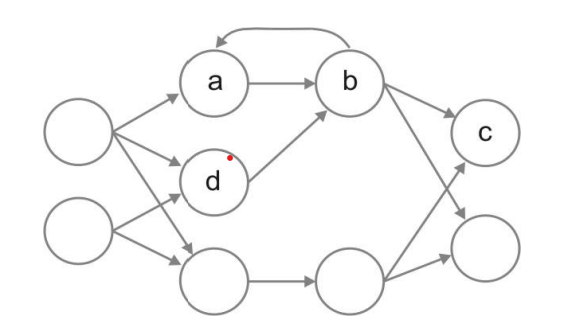
\includegraphics[width=0.8\textwidth]{images/nn-povratna-veza}
    \caption{Mreža s povratnom vezom
    \protect\footnotemark}
    \label{fig:slika5}
\end{figure}
\FloatBarrier
\footnotetext{\url{https://www.ibm.com/topics/neural-networks}}

\pagebreak
Lateralno povezane mreže predstavljaju neuronske mreže gdje neuroni u istom sloju međusobno komuniciraju.
Često se koristi kako bi se omogućila suradnja između neurona kako bi se pojačale određene značajke unutar sloja.
\FloatBarrier
\begin{figure}[h]
    \centering
    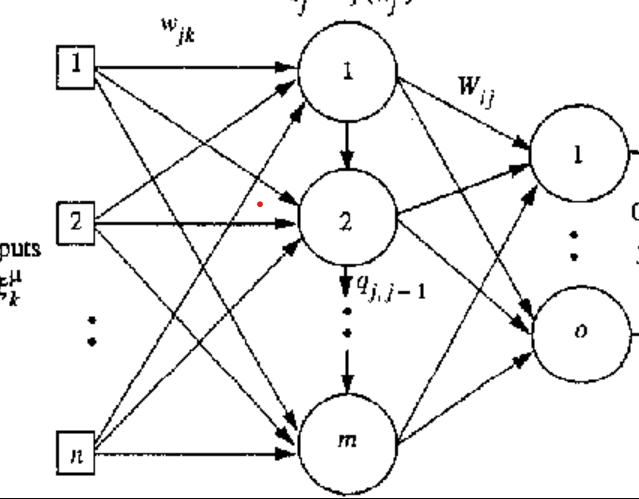
\includegraphics[width=0.8\textwidth]{images/Lateral-connected-nn}
    \caption{Lateralno povezana mreža
    \protect\footnotemark}
    \label{fig:slika6}
\end{figure}
\FloatBarrier
\footnotetext{\url{https://ai.stackexchange.com/questions/34054/what-is-meant-by-lateral-connection-in-the-context-of-neural-networks}}


\section{Backpropagation}\label{sec:backpropagation}
Backpropagation ili postupak propagacije pogreške unatrag je postupak učenja neuronskih mreža koji se temelji na učinkovitom izračunu svih parcijalnih derivacija
i njihovoj primjeni na određivanje iznosa kojim korigiramo svaku od težina.
Algoritam koristi metodu gradijentnog spusta kako bi minimizirao nastalu pogrešku.
Za neuronsku mrežu koja u izlaznom sloju ima \textit{k} izlaznih neurona i za skup za učenje \textit{D}, ukupna empirijska pogreška iznosi:
\begin{align*}
    E(\vec{w}) &= \frac{1}{2N} \sum_{d \in D} \sum_{k \in K} (t_{kd} - o_{kd})^2
\end{align*}
gdje je $t_{kd}$ ciljna ili očekivana vrijednost izlaza, a $o_{kd}$ je stvarna izlazna vrijednost, odnosno vrijednost izlaza neurona.
Algoritam propagacije pogreške unatrag je sljedeći:
\begin{enumerate}
    \item Postavimo početne težine na neke slučajno odabrane vrijednosti
    \item Ponavaljamo postupak dok nije zadovoljen uvjet zaustavljanja
    \begin{itemize}
        \item Postavimo podatke za primjer \textit{i} na ulaz mreže
        \item Izračunamo izlaze svih neurona u svakom sloju
        \item Odredimo pogrešku \textit{i}-tog neurona na izlaznom sloju prema sljedećem izrazu
        \begin{align*}
            \delta_{i}^{K} &= o_{s,i} \cdot (1 - o_{s,i}) \cdot (t_{s,i} - o_{s,i})
        \end{align*}
        gdje nam izraz $o_{s,i}$ * (1 - $o_{s,i}$) označava parcijalnu derivaciju prijenosne funkcije, koja je u ovom primjeru sigmoidalna prijenosna funkcija.
        Izraz ($t_{s,i}$ - $o_{s,i}$) odgovara razlici ciljne i dobivene vrijednosti.
        \item Nakon toga se vraćamo sloj po sloj prema početku neuronske mreže odnosno ulaznom sloju.
        Sada je potrebno za svaki neuron \textit{i} u svakom sloju \textit{k} izračunati njegovu pogrešku.
        To radimo pomoću sljedećeg izraza:
        \begin{align*}
            \delta_{i}^{(k)} &= y_{i}^{k} \cdot (1 - y_{i}^{k}) \left(\sum_{d \in D} w_{i,d} \cdot \delta_{d}^{k+1}\right)
        \end{align*}
        Opet prepoznajemo derivaciju sigmoidalne prijenosne funkcije, a drugi dio izraza odgovara težinskoj sumi pogrešaka neurona kojem on šalje svoj izlaz.
        Bolje rečeno zbraja sve pogreške neurona na čiji ulaz utječe trenutni neuron pomnožen s težinskim faktorom.
        Težinski faktor pokazuje koliko je taj neuron utjecao na iznos pogreške za neuron \textit{s}.
        \item Nakon toga radimo korekciju tezine $w_{i,j}^k$ prema izrazu:
        \begin{align*}
            w_{i,j}^{(k)} \leftarrow w_{i,j}^{(k)} + \eta \cdot y_{i}^k \cdot \delta_{j}^{k+1}\right)
        \end{align*}
        gdje nam je \textit{$\eta$} stopa učenja, \textit{$y_{i}^k$} izlaz neurona i u k-tom sloju, a \textit{$\delta_{j}^{k+1}$} pogreška neurona u sljedećem sloju
    \end{itemize}
\end{enumerate}
Kao što se može vidjeti, naziv algoritma je prikladan jer prvo moramo odrediti izlaz mreže, a nakon toga idemo od izlaznog sloja prema ulaznom sloju i računamo pogrešku neurona u svakom sloju od izlaznog prema ulaznom sloju te korigiramo težine.
    %! Author = Dean
%! Date = 12/28/2023

\chapter{Evolucija konvolucijskih neuronskih mreža}\label{ch:evolucija-konvolucijskih-neuronskih-mreza}
Konvolucijske neuronske mreže \emph{KNM} predstavlja ključnu inovaciju u području analize slika i obrade vizualnih podataka.
U posljednjem razdoblju, KNM arhitektura doživjela je značajan tehnološki napredak.
Ovaj napredak omogućio je postizanje rezultata koji su prije bili nezamislivi, često se približavajući ili čak nadmašujući ljudske sposobnosti u određenim zadacima vizualne analize.
Današnje vrijeme karakterizira raznolikost KNM-ova, s različitim arhitekturama koje su prilagođene specifičnim zadatcima.
Svaka arhitektura ima svoje prednosti i mane, a \enquote{Teorem besplatnog ručka} ukazuje na to da nema univerzalno najbolje arhitekture.
Zato ćemo sada malo proći kroz evoluciju konvolucijskih neuronskih mreža od samih početaka pa do danas.

\section{Neocognitron}\label{sec:neocognitron}
Možemo reći da je Neocognitron preteča konvolucijskih neuronskih mreža.
Ova arhitektura je prva uvela pojmove kao što su ekstrakcija značajki (\emph{feature extraction}), konvolucija (\emph{convolution}), i slojevi uzorkovanja (\emph{pooling layers}).
\FloatBarrier
\begin{figure}[h]
    \centering
    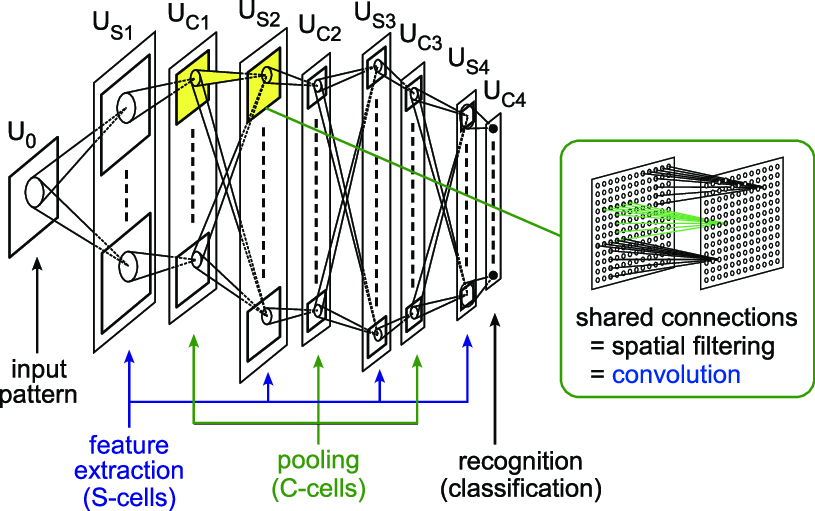
\includegraphics[width=0.6\textwidth]{images/Neocognitron}
    \caption{Arhitektura Neocognitron}
    \label{fig:slika7}
\end{figure}
\FloatBarrier
Arhitektura Neocognitrona sastoji se od alternirajućih S i C slojeva, pri čemu svaki od njih sadrži S i C stanice.
S stanice, ili jednostavne stanice, služe za detekciju lokalnih značajki, dok C stanice, ili kompleksne stanice, služe za dodavanje tolerancije prema samoj poziciji objekta.
Na taj način dobivamo model koji je invarijantan na translacijske promjene, odnosno trebao bi prepoznati oblik bez obzira na to gdje se nalazi na slici.

\section{LeNet-5}\label{sec:lenet-5}
LeNet-5 je dizajnirana od strane francuskog informatičara Yanna LeCuna između 1989. i 1998. godine i postigla je uspjeh u prepoznavanju rukom pisanih brojeva.

Arhitektura se sastojala od tri konvolucijska sloja i dva sloja za uzrokovanje koji su bili međusobno alternirajući. Na kraju su se nalazila dva potpuno povezana sloja.

U konvolucijskim slojevima koristio se 5x5 filter s korakom veličine 1, odnosno s pomakom veličine 1. S druge strane, slojevi za uzrokovanje bili su 2x2 s pomakom veličine 2.
\begin{figure}[h]
    \centering
    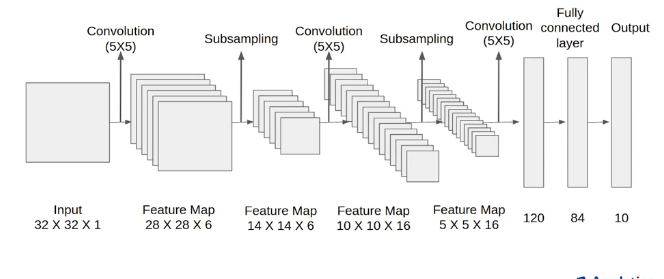
\includegraphics[width=0.6\textwidth]{images/LeNet}
    \caption{Arhitektura LeNet-5.}
    \label{fig:slika8}
\end{figure}
Dimenzija ulazne slike je 32x32x1 jer se ova arhitektura uglavnom koristila za prepoznavanje rukom pisanih brojeva. Dimenzije označavaju širinu, visinu i dubinu slike. Za crno-bijele slike dubina je 1, što znači da postoji samo jedan kanal. Za RGB slike, dubina bi bila 3 (jedan kanal za crvenu, zelenu i plavu komponentu svake boje).

Prvi konvolucijski sloj ima 6 filtera veličine 5x5 s pomakom od 1.
Rezultat tog sloja je značajka veličine 28x28x6.
Izlazni sloj se može izračunati pomoću formule: \[ \textit{dimenzija} = \frac{\textit{ulazna dimenzija} - \textit{veličina filtera}}{\textit{korak}} + 1 \].

Nakon toga slijedi sloj za uzrokovanje veličine 2x2.
Ovdje se koristi average pooling koji za vrijednost uzima prosjek od odabrane 4 vrijednosti.

Dalje slijede još dva konvolucijska sloja, jedan sloj za uzrokovanje i dva potpuno povezana sloja, od kojih je jedan izlazni sloj.
Izlazni sloj sastoji se od 10 neurona i koristi Softmax kao aktivacijsku funkciju.
Softmax je prikladan jer za svaku klasu daje vjerojatnost da ulaz pripada toj klasi, a predikcija se izvodi tako da se odabere klasa s najvećom vjerojatnošću.

\section{AlexNet}\label{sec:alexnet}
AlexNet je arhitektura konvolucijske neuronske mreže koja se primarno koristi za klasifikaciju slika. Koristi 5 konvolucijskih slojeva u kombinaciji s max poolingom, a na kraju ima 3 potpuno povezana sloja. Kao aktivacijsku funkciju koristi ReLU, osim na izlaznom sloju gdje se i dalje koristi Softmax. Primjenom ReLU aktivacije uspjeli su ubrzati proces treniranja čak 6 puta.

Za razliku od LeNet-5 modela, ulaz u AlexNet je RGB slika dimenzija 227x227.
\FloatBarrier
\begin{figure}[h]
    \centering
    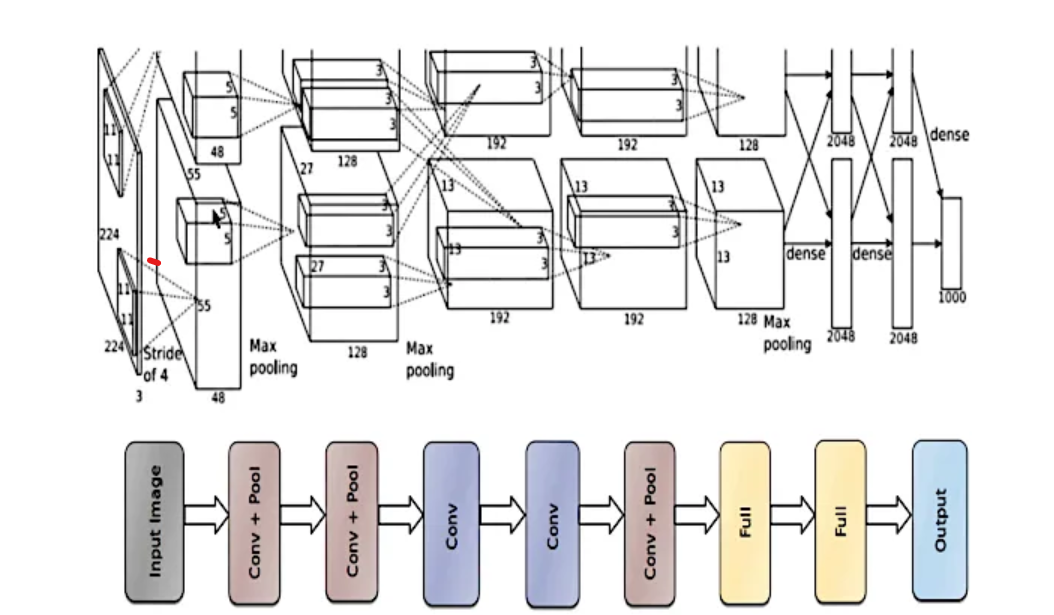
\includegraphics[width=0.6\textwidth]{images/AlexNet}
    \caption{Arhitektura AlexNet}
    \label{fig:slika9}
\end{figure}
\FloatBarrier

Ako pogledamo arhitekturu, primjećujemo da se broj filtera povećava kako dublje idemo u mrežu, što znači da se može izvući više značajki.
Također, veličina filtra se smanjuje kako dublje ulazimo u mrežu.
Mreža se sastoji od 62.3 miliona parametara, za usporedbu LeNet-5 ima 60000.
Zbog ogromne količine parametara, moramo paziti da nam model ne postane prenaučen te se u tu svrhu koristi regularizacija.
Kod AlexNet-a za regularizaciju se koristi takozvani dropout.
Ideja dropout-a je jednostovna: tijekom treninga, nasumično se \enquot{isključuju} određeni neuroni u mreži i ona su privremena i mijenjaju se u svakoj iteraciji treninga.
Samim time što tijekom treninga mi isključimo jedan dio neurona, dovodi mrežu u situaciju da smanjuje međuovisnost o neuronima, da se prilagodi različitim kombinacijama neurona koji su prisutni.
Kao uvijek imamo i šumove u podatcima, a pomoću dropout-a mi sprečavamo memorizaciju šumova što pomaže da model bolje generalizira.
Naravno tijekom testiranja dropout se ne radi.

\section{VGGNet}\label{sec:vggnet}
VGGNet arhitektura je razvijena od strane Visual Geometry Group na Sveučilištu Oxford.
Grupa je radila s pretpostavkom da dublje strukture konvolucijskih mreža mogu bolje modelirati nelinearnosti.

\FloatBarrier
\begin{figure}[h]
    \centering
    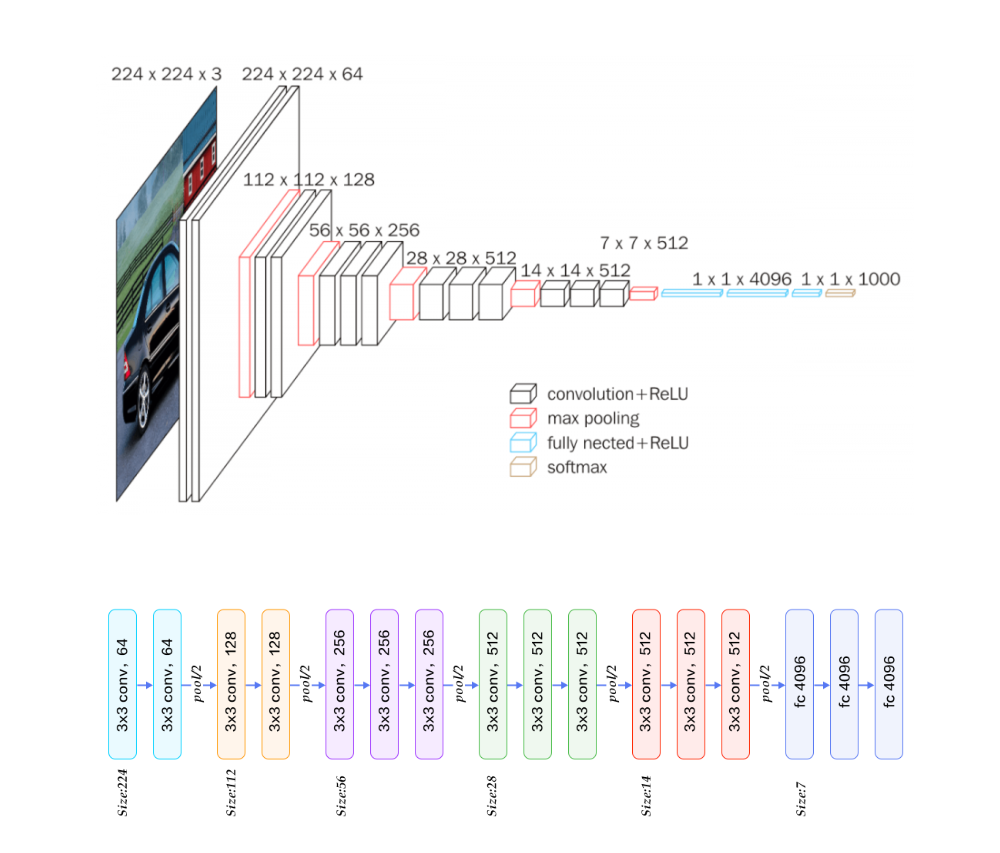
\includegraphics[width=0.6\textwidth]{images/VGGNet}
    \caption{Arhitektura VGGNet}
    \label{fig:slika10}
\end{figure}
\FloatBarrier

Ulaz u mrežu je RGB slika dimenzija 224x224.
Imamo modele čija se dubina razlikuje u rasponu od VGG11 do VGG19, gdje je VGG11 se sastoji od 8 konvolucijskih slojeva i 3 potpuno povezana sloja, dok VGG19 se sastoji od 16 konvolucijsih i 3 potpuno povezana sloja.
Da bi smanjili broj parametara, odlučili su postaviti veličinu filtra na 3x3 za svaki sloj u mreži.
Ali i sa tom modifikacijom model će imati ogroman broj parametara.
Recimo VGG16 će u konačnici imati 138357544 parametara.
Za treniranje se koristi gradijentni spust s momentom \emph{0.9}.
Kao regularizaciju koristi L2 regularizaciju i dropout koji se koristi nakon drugog potpuno povezanog sloja s vrijednosti od 50\%.


    %! Author = Dean
%! Date = 12/30/2023

\chapter{Komponente konvolucijskih neuronskih mreža}\label{ch:komponente-konvolucijskih-neuronskih-mreza}
Konvolucijske neuronske mreže, baš kao i obične neuronske mreže, sastoje se od ulaznog sloja, izlaznog sloja i skrivenih slojeva.
U matematičkom smislu, konvolucija predstavlja proces kombiniranja dviju funkcija kako bi se generirala treća funkcija poznata kao izlazna funkcija.

\section{Konvolucijski sloj}\label{sec:konvolucijski-sloj}
Jedan od glavnih gradivnih blokova konvolucijske neuronske mreže je konvolucijski sloj.
Sloj se sastoji od ulaznih vektora, izlaznih vektora ili mapa značajki i sastoji se od filtra ili kernela.
Filtri su uglavnom male matrice veličine 3x3, 5x5 ili 1x1, a sami filtri služe da izvuču bitne informacije \emph{značajke} iz ulaznih vektora.
Iz tog razloga, neće imati samo jedan filter, jer s jednim filtrom ne mogu se izvući sve potrebne značajke.
Filtar se primjenjuje na ulazne podatke tako što pomnoži elemente na istim pozicijama i sumira njihove vrijednosti.
Taj proces je poznat kao konvolucija.

\FloatBarrier
\begin{figure}[h]
    \centering
    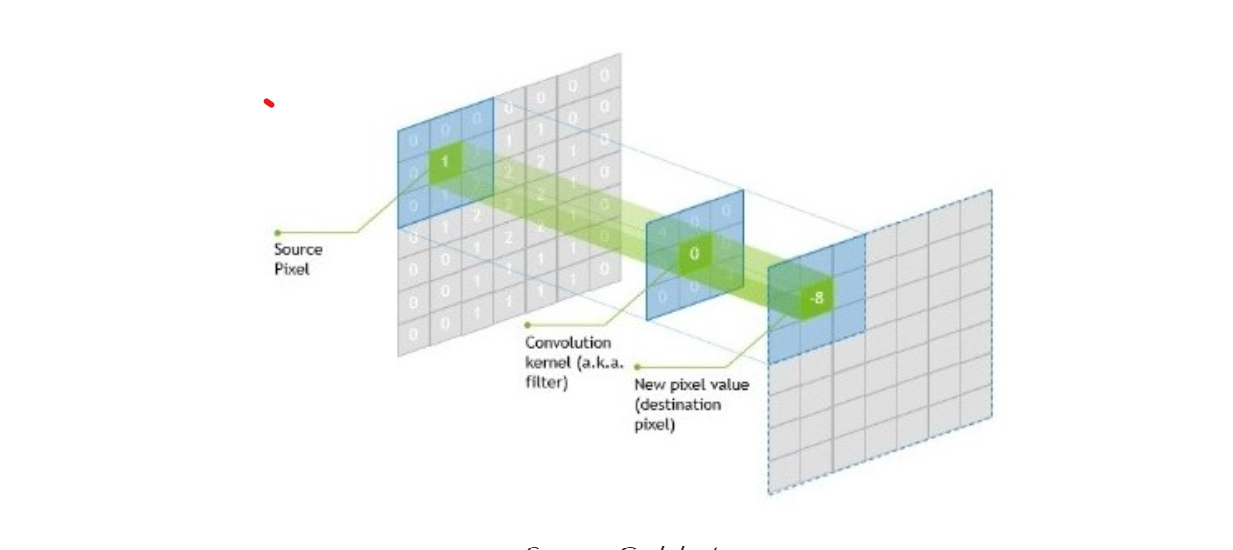
\includegraphics[width=0.7\textwidth]{images/Convolution}
    \caption{Konvolucijski sloj
    \protect\footnotemark}
    \label{fig:slika13}
\end{figure}
\FloatBarrier

\footnotetext{\url{https://www.analyticsvidhya.com/blog/2022/03/basics-of-cnn-in-deep-learning/}}

U konvolucijskom sloju koristimo nadopunjavanje \emph{padding} i korak \emph{stride}, a oni zapravo određuju kako će se prevesti konvolucija ulaznih podataka i dimenzija izlaza.
Za njih možemo reći da su hiperparametri.

Korak nam govori kako filtar primjenjujemo na ulaznu matricu, odnosno kako se krećemo po matrici po stupcima.
Ako postavimo korak na 1, filtar će se pomaknuti za 1 stupac u lijevo do kraja, dok će se s korakom 2 pomaknuti za 2 stupca.
Jasno je da veći korak rezultira manjom dimenzijom izlaza, i obrnuto.
\FloatBarrier
\begin{figure}[h]
    \centering
    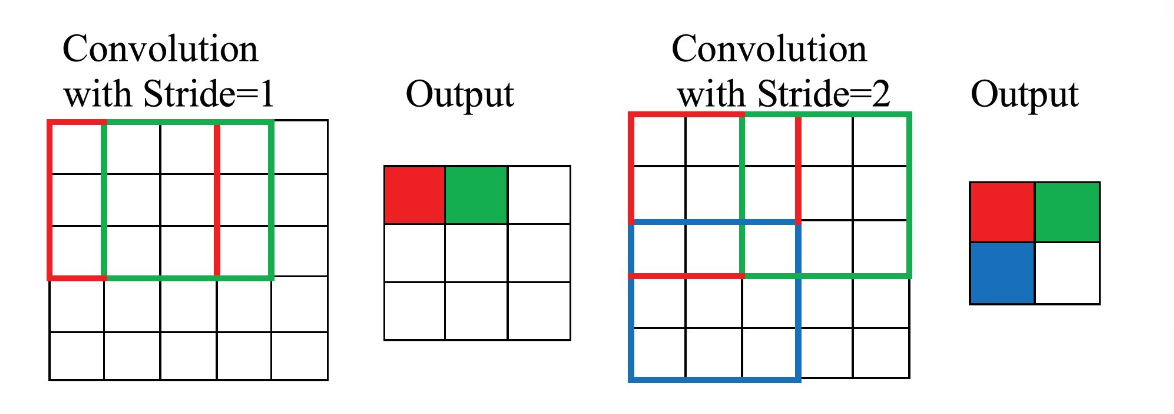
\includegraphics[width=0.7\textwidth]{images/Stride}
    \caption{Učinak različitih vrijednosti koraka \emph{stride}
    \protect\footnotemark}
    \label{fig:slika14}
\end{figure}
\FloatBarrier
\footnotetext{\url{https://www.analyticsvidhya.com/blog/2022/03/basics-of-cnn-in-deep-learning/}}


Problem je što na ovaj način možemo izgubiti potrebne informacije, a i informacije koje se nalaze na samom rubu i u kutovima se puno manje koriste.
Zbog toga imamo takozvani \enquote{padding}, što je zapravo proces nadopunjavanja ulazne matrice.
Postoje dvije tehnike nadopunjavanja: bez nadopunjavanja (\emph{valid padding}) i nadopunjavanje istom količinom (\emph{same padding}).
U tehnici \emph{valid padding}, zapravo se ne radi ništa i dozvoljava se da se dimenzija izlaza smanji, dok se u \emph{same padding} tehnici dodaju dodatni redci i stupci, popunjeni nulama, kako bi dimenzija izlaza bila očuvana i kako bi se više značaja pridalo originalnim rubnim pozicijama.

\FloatBarrier
\begin{figure}[h]
    \centering
    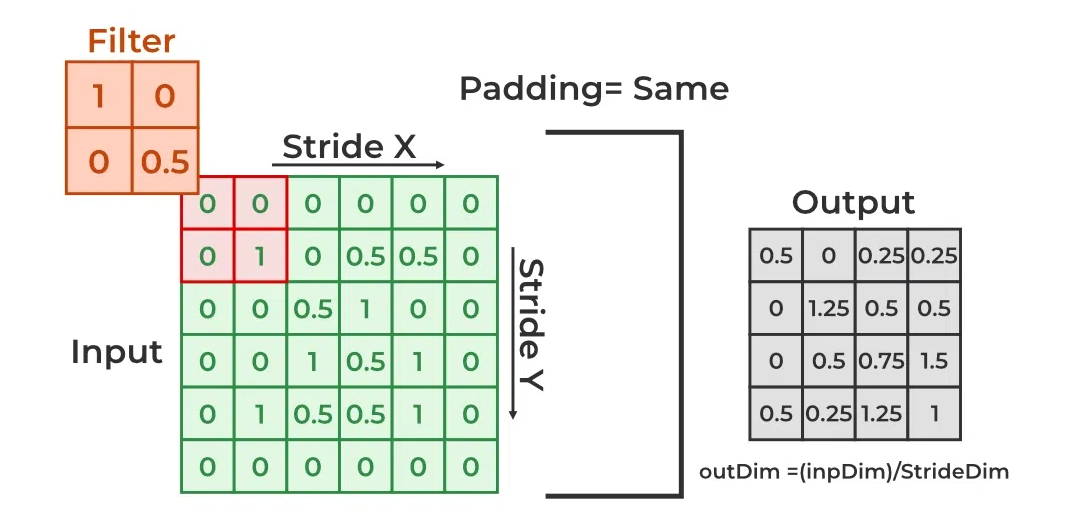
\includegraphics[width=0.6\textwidth]{images/Padding}
    \caption{Učinak nadopunjavanja \emph{same padding}
    \protect\footnotemark}
    \label{fig:slika15}
\end{figure}
\FloatBarrier
\footnotetext{\url{https://www.geeksforgeeks.org/cnn-introduction-to-padding/}}


\section{Sloj uzrokovanja}\label{sec:sloj-uzrokovanja}
Uloga ovog sloja je postupno smanjiti dimenzije svake značajke, odnosno izlaza konvolucijskog sloja, i na taj način smanjiti broj parametara.
Obično se sloj za uzrokovanje radi s matricom 2x2.

\FloatBarrier
\begin{figure}[h]
    \centering
    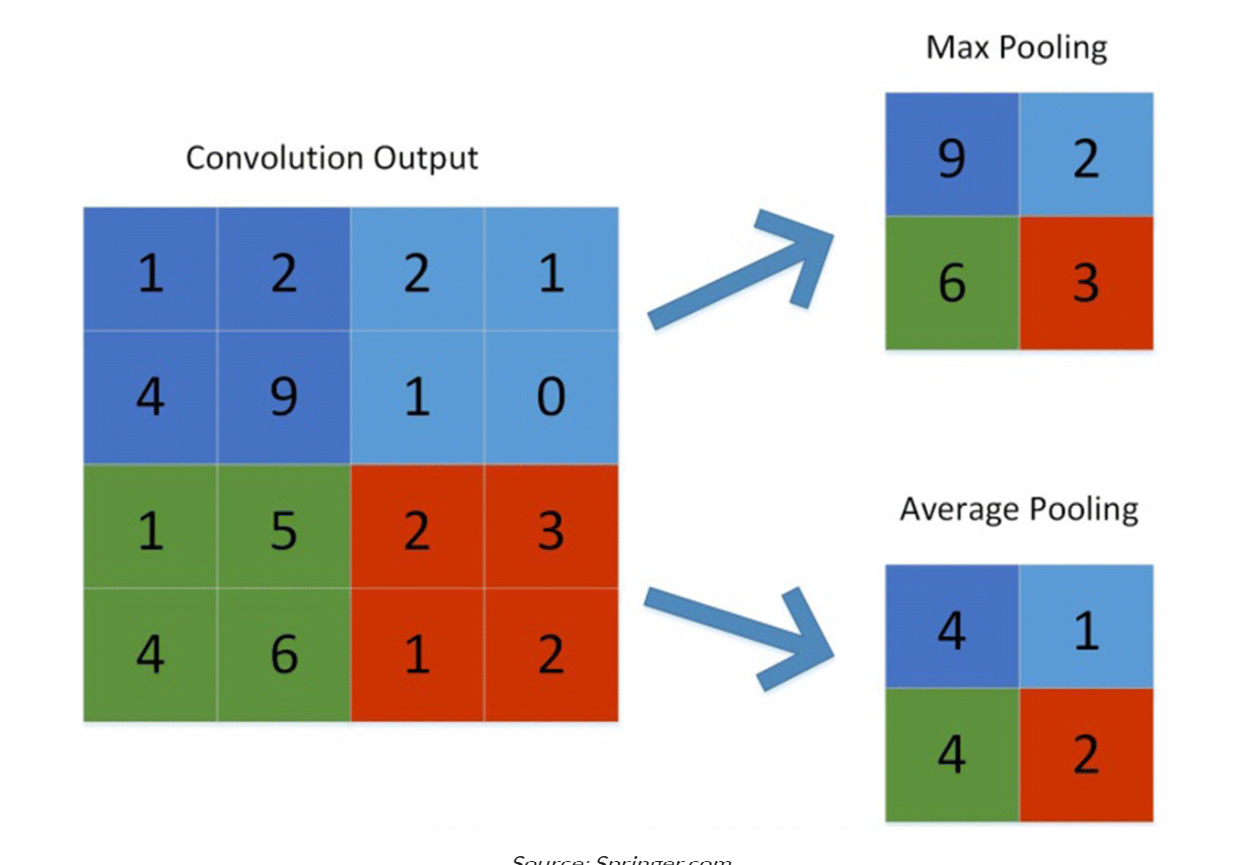
\includegraphics[width=0.7\textwidth]{images/Pooling}
    \caption{Prikaz \emph{max padding-a} i \emph{average padding-a}
    \protect\footnotemark}
    \label{fig:slika16}
\end{figure}
\FloatBarrier
\footnotetext{\url{https://www.geeksforgeeks.org/cnn-introduction-to-padding/}}


Postoje dvije metode za uzrokovanje: \emph{average pooling} metoda računa prosjek elemenata u matrici, dok \emph{max pooling} metoda, češće korištena, uzima element s najvećom vrijednošću.
Što je veća matrica za uzrokovanje, to će dimenzije biti manje, i obrnuto.

\section{Potpuno povezani sloj}\label{sec:potpuno-povezani-sloj}
Potpuno povezani sloj zapravo je unaprijedna neuronska mreža.
Njezin ulaz je izlaz konvolucijskog sloja ili sloja za uzrokovanje, a kako bismo te izlaze mogli unijeti kao ulaz u neuronsku mrežu, prvo moramo matricu pretvoriti u vektor.
Nakon toga imamo niz skrivenih slojeva u neuronskoj mreži, a na kraju imamo izlazni sloj koji će dati rezultat cijelog ovog procesa.
    %! Author = Dean
%! Date = 12/16/2023

\chapter{Arhtekture konvolucijskih neuronskih mreža}\label{ch:arhtekture-konvolucijskih-neuronskih-mreza}

    %! Author = Dean
%! Date = 12/30/2023

\chapter{Treniranje i optimizacija}\label{ch:treniranje-i-optimizacija}

Kao što smo vidjeli ranije, konvolucijske neuronske mreže imaju ogromnu količinu parametara, a da bi naš model bio što točniji moramo mu postaviti ispravne parametre a to postižemo treniranjem.
Da bi mogli uopće trenirati mrežu, trebaju nam podatci nad kojim ćemo ga trenirati.
Kako ne bi pretrenirali model, podatke dijelimo na testne podatke i podatke za ispitivanje u omjeru 70% za treniranje i 30% za testiranje.
Svrha podjele je istrenirati mrežu nad testnim podatcima, a zatim, na temelju rezultata nad podatcima za ispitivanje, podesiti hiperparametre ako je potrebno kako bi se poboljšala generalizacija modela.
Proces treniranja koristi propagaciju greške unatrag, koji smo obradili ranije.

Imamo razne načine optimiranja, ali ovdje ću obraditi najjednostavniji - gradijentni spust.
Ideja iza gradijentnog spusta je pronaći minimum funkcije gubitka iterativnim izračunavanjem gradijenta i kretanjem prema njemu.
Problem kod ovog načina je ako funkcija gubitka nije konveksna, odnosno ako ima lokalnih minimuma, gdje gradijentni spust može zapeti.
Osim toga, nemamo određenu početnu točku već ju nasumično biramo, pa vrijeme i točnost modela ovise o početnoj točki.

\FloatBarrier
\begin{figure}[h]
    \centering
    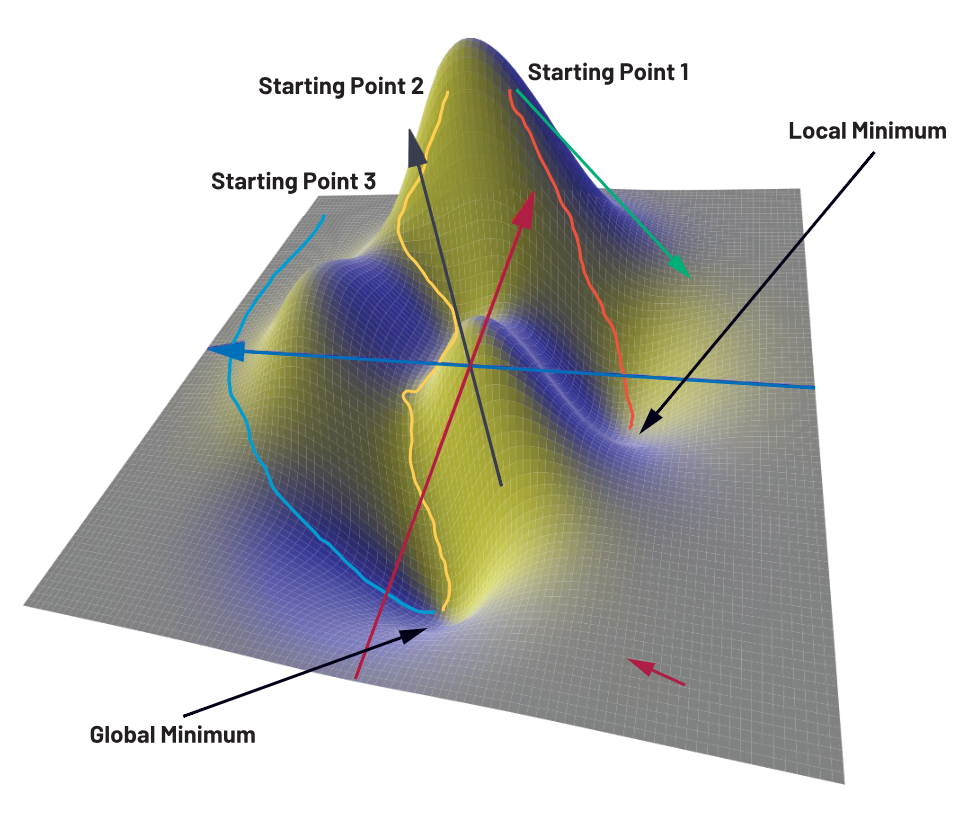
\includegraphics[width=0.8\textwidth]{images/Gradijentni-spust}
    \caption{Gradijentni spust}
    \label{fig:slika18}
\end{figure}
\FloatBarrier

Često do loše generalizacije dolazi zato što nam je model presložen, što znači da se lako prilagodi šumovima koji se nalaze u testnim podatcima.
Zato se u optimizaciju uvodi regularizacija.
Regularizacija nam omogućava da krenemo od vrlo složenog modela i onda će nam sama regularizacija tijekom treniranja smanjivati složenost modela.
L2 i L1 regularizacija je popularna i ona se direktno može ubaciti u funkciju gubitka, ali puno češće se koristi tehnika koju smo već objasnili a to je \emph{dropout}.
Važno je napomenuti da treba biti oprezan pri odabiru jačine regularizacije, jer ako je prejaka regularizacija model će biti prejednostavan, podnaučen model, te će isto loše generalizirati.
Isto tako slaba regularizacija neće uopće utjecat na složenost modela te će se model opet prilagodit šumovima i dobit ćemo prenaučen model.
Tako da za dropout metodu treba pažljivo odabrati hiperparametar p koji govori koliko će neurona \enquote{ugasiti} tijekom jedne iteracije treniranja.
    %! Author = Dean
%! Date = 12/16/2023

\chapter{Transfer Learning}\label{ch:transfer-learning}
    %! Author = Dean
%! Date = 12/30/2023

\chapter{Primjena konvolucijskih neuronskih mreža}\label{ch:primjena-konvolucijskih-neuronskih-mreza}

Konvolucijske neuronske mreže koriste se u području računalnog vida i prepoznavanja slika.
Glavna zaduženja u tom procesu obuhvaćaju prepoznavanje objekata, grupiranje objekata te interpretaciju onoga što slika prikazuje.

Osim toga, konvolucijske neuronske mreže često se primjenjuju u algoritmima preporuka.
Primjerice, na web trgovinama možemo vidjeti preporuke proizvoda koji bi nas mogli zanimati, temeljene na našem prethodnom ponašanju na platformi.

Jedno od najpopularnijih područja primjene konvolucijskih mreža danas je prepoznavanje lica.
To se široko koristi na socijalnim mrežama, u nadzornim sustavima, ali i u svrhu sigurnosti jer se temelji na identifikaciji korisnika putem prepoznavanja lica.
Socijalne mreže često koriste tehnologiju prepoznavanja lica kako bi olakšale označavanje ljudi na fotografijama ili primijenile različite filtre za transformaciju lica u kreativne i zabavne sadržaje.

No, primjena konvolucijskih mreža nije ograničena na zabavu i oglašavanje.
U medicini se također široko koriste, posebno u detekciji anomalija na magnetskim rezonancijskim slikama.

Također, konvolucijske neuronske mreže koriste se u autonomnim vozilima za prepoznavanje pješaka, vozila i drugih objekata na cestama.
Ova tehnologija ima ključnu ulogu u razvoju sigurnijih i učinkovitijih sustava samovozećih vozila.

U području znanstvenih istraživanja, konvolucijske mreže primjenjuju se za analizu kompleksnih podataka, poput astrofotografija, bioloških uzoraka i drugih znanstvenih slika.
Ova primjena omogućuje automatiziranu analizu i izvlačenje značajki iz ogromnih skupova podataka.

Ove primjene ilustriraju široki spektar mogućnosti konvolucijskih neuronskih mreža u različitim sektorima, pokazujći njihovu snažnu ulogu u analizi i interpretaciji vizualnih podataka.
    %! Author = Dean
%! Date = 12/30/2023

\chapter{Zaključak}\label{ch:zakljucak}
Unatoč imresivnim rezultatima, konvolucijske neuronske mreže suočavaju se s izazovima kao što je potreba za velikim skupom podataka i velika računalna moć.
Budući smjerovi istraživanja usmjereni su prema poboljšanju efikasnosti modela i razvoju tehnologije \emph{transfer learninga}.
Razumijevanje tih izazova i rad na njihovom rješavanju su ključni za daljni napredak konvolucijskih neuronskih mreža.
    %! Author = Dean
%! Date = 12/16/2023

\begin{thebibliography}{9}
\end
\bibliographystyle{fer}


\end{document}
